\documentclass[journal, twocolumn]{IEEEtran}

\usepackage{cite}
\usepackage{amsmath,amssymb,amsfonts}
\usepackage{algorithmic}
\usepackage{graphicx}
\usepackage{textcomp}
\usepackage{xcolor}
\usepackage{booktabs}
\usepackage{multirow}

\begin{document}

\title{Breaking the Affective Invariance Assumption: A Distribution-Level Analysis of Physiological and Subjective Divergence}

\author{
    \IEEEauthorblockN{Kotaro Furukawa, \textit{Student Member, IEEE}}\\
    \IEEEauthorblockA{Frontier School of Transdisciplinary Sciences, Kanazawa University, Ishikawa, Japan\\
    Email: f.kotaro.0530@gmail.com}
}

\maketitle

\begin{abstract}
Emotion recognition from physiological signals fundamentally relies on the implicitly assumed invariance of the mapping from autonomic physiological state to subjective emotional experience (e.g., that an elevated heart rate universally equates to stress). However, human affective meaning is profoundly context-dependent. The prevalent methodology of interpolating discrete, block-level subjective labels across continuous, high-resolution physiological sensor data severely compromises ecological validity and artificially inflates predictive performance. In this letter, we rigorously re-evaluate the widely used Wearable Stress and Affect Detection (WESAD) dataset by deliberately eliminating instantaneous label interpolation. Utilizing 100 Hz high-resolution, 4-dimensional physiological feature extraction (EDA Tonic/Phasic components and HRV LF/HF bands) via convex optimization and continuous wavelet transforms, we introduce a method to calculate the mathematical distribution overlap between distinct contextual tasks at the macro-level. Our results demonstrate that for a significant subset of individuals (roughly 27\%), over 87\% of the continuous physiological signal space during an acute stress task is mathematically enveloped within their physiological distribution during a baseline resting task, despite these individuals reporting highly polarized subjective Self-Assessment Manikin (SAM) scores. These findings provide critical empirical evidence that isolated physiological sensing without holistic context integration is insufficient for deterministic affective state prediction, urging a paradigm shift toward ``meaning-oriented'' interactive sensing frameworks.
\end{abstract}

\begin{IEEEkeywords}
Affective Computing, Electrodermal Activity (EDA), Heart Rate Variability (HRV), Context-Awareness, Wearable Sensors.
\end{IEEEkeywords}

\section{Introduction}
\IEEEPARstart{T}{he} predominant paradigm in affective computing and ubiquitous sensing heavily relies upon predictive modeling architectures aimed at mapping physiological sensor data to psychological states \cite{picard1997}. Contemporary wearable systems leveraging electrocardiography (ECG) and electrodermal activity (EDA) operate under a core assumption of physiological invariance ($X \rightarrow Y$); they frequently presume that the manifestation of specific autonomic reactions, such as increased sympathetic arousal, corresponds uniquely to predefined affective constructs like ``Stress'' or ``Anxiety'' \cite{schmidt2018wesad}.

This state-determination approach has achieved high classification accuracies in controlled laboratory environments. However, a fundamental methodological flaw permeates the supervised learning pipelines of numerous studies utilizing physiological datasets: instantaneous label interpolation. Because continuous ground-truth reporting of subjective emotion imposes severe cognitive loads on participants, researchers routinely utilize block-level, post-task questionnaires (e.g., the Self-Assessment Manikin (SAM) \cite{bradley1994}). These singular, retrospective scores are then broadcasted across tens of thousands of continuous, high-resolution sensor data points collected during the prior temporal block. This practice implicitly assumes that the subject's affective state remained perfectly static and invariant at the intra-block microsecond level, essentially assigning artificial, fabricated meaning to instantaneous psychophysiological micro-fluctuations and destroying the ecological validity of the dynamic emotional experience \cite{wilhelm2006}.

When deployed in the wild, systems trained on such interpolated data frequently fail because they ignore the profound context-dependency of human emotion \cite{barrett2017}. The identical autonomic response (e.g., a racing heart and increased sweating) can be subjectively experienced as crippling anxiety before a public speech, or as exhilarating flow during competitive sports.

This letter proposes an alternative validation framework to critically examine the stability of predictive physiological sensing. We completely discard point-level label interpolation. Instead, we isolate entire blocks of task data and compare their multi-dimensional physiological distributions natively. By calculating the physical overlap of these distributions, we demonstrate that identical physiological responses routinely map to drastically different subjective meanings. Our contributions are summarized as follows:
\begin{itemize}
    \item We present a rigorous signal processing pipeline extracting 100 Hz continuous features from the WESAD dataset without reliance on interpolated affective labels.
    \item We introduce a distribution-level mathematical overlap metric ($\Omega$), demonstrating that up to 98.6\% of stress-induced physiological responses can be statistically indistinguishable from baseline states for certain individuals.
    \item We provide empirical proof of the failure of the invariance assumption, demanding a transition from predictive ``state determination'' toward ``meaning-oriented'' frameworks.
\end{itemize}

\section{Methodology}

\subsection{Dataset and Ground Truth Segregation}
We acquired raw physiological signals from the Wearable Stress and Affect Detection (WESAD) dataset \cite{schmidt2018wesad}, a benchmark corpus for multimodal affect detection. We utilized data from 15 subjects, isolating two distinct condition blocks: the ``Baseline'' task (neutral reading, $\approx$ 20 minutes) and the ``Stress'' task (the Trier Social Stress Test, $\approx$ 10 minutes). 

Crucially, we rejected continuous labelling. Ground truth subjective affective states were established strictly at the holistic block level utilizing the subjects' self-reported Valence (1-9) and Arousal (1-9) SAM scores recorded post-task.

\subsection{Ultra-High Resolution Signal Processing}
To prevent temporal data obfuscation resulting from coarse rolling-window averages (e.g., typical 60-second block means), we reconstructed the physiological footprint natively at a 100 Hz continuous resolution.

\subsubsection{Electrodermal Activity (EDA)}
We up-sampled the 4 Hz wrist EDA signal ($y$) to 100 Hz utilizing cubic spline interpolation. We then applied the continuous-time convex optimization approach (cvxEDA) \cite{cvxeda2015} to decompose the raw EDA signal into its independent background tonic level ($t_{level}$) and impulsive sudomotor bursts ($p$). 
The model defines EDA as:
\begin{equation}
    y = H \cdot p + t_{level} + \epsilon
\end{equation}
where $H$ is the sudomotor nerve impulse response. The separated continuous vectors, $EDA_{Tonic}$ and $EDA_{Phasic}$, were extracted for each 0.01s epoch.

\subsubsection{Heart Rate Variability (HRV)}
R-R wave intervals (RRI) were reconstructed into a continuous 100 Hz timescale. Because traditional Fast Fourier Transforms depend on broad stationary assumptions unsuited for volatile affective states, we utilized a Continuous Wavelet Transform (CWT) with an analytic Morlet wavelet to extract instantaneous band powers:
\begin{equation}
    W(a, \tau) = \frac{1}{\sqrt{a}} \int x(t) \psi^*\left(\frac{t - \tau}{a}\right) dt
\end{equation}
The instantaneous Low-Frequency ($HRV_{LF}$, 0.04-0.15 Hz) and High-Frequency ($HRV_{HF}$, 0.15-0.4 Hz) powers were computed.

\subsection{Distribution-Level Overlap Computation}
This pipeline yielded a continuous 4-dimensional physiological space $X = [EDA_{Tonic}, EDA_{Phasic}, HRV_{LF}, HRV_{HF}]$. Let $S_{base}^{(i)}$ and $S_{stress}^{(i)}$ denote the entire set of physiological points for subject $i$ during the baseline and stress blocks, respectively.
Data for each subject were z-score normalized corresponding to their individual baseline mean $\mu_{base}^{(i)}$ and standard deviation $\sigma_{base}^{(i)}$. 

We defined the Distribution Overlap Density ($\Omega$) as the percentage of points in the Stress block that reside within a densely populated local neighborhood of the Baseline block. Utilizing a Nearest Neighbors search configured to a strict Euclidean radius of $R = 1.0\sigma$:
\begin{equation}
    \Omega^{(i)} = \frac{100}{|S_{stress}^{(i)}|} \sum_{x \in S_{stress}^{(i)}} \mathbb{I}\left(\min_{x' \in S_{base}^{(i)}} \| x - x' \|_2 \leq R\right)
\end{equation}
where $\mathbb{I}(\cdot)$ is the indicator function. A high $\Omega$ value signifies that the physiological reality of the stress task is topologically engulfed by the baseline state.

\section{Results}

\subsection{Convergence of State vs. Divergence of Meaning}
We primarily analyzed Subject 11 (S11), who exhibited highly polarized block-level SAM scores: Valence 6 / Arousal 4 during Baseline (positive, neutral arousal) and Valence 2 / Arousal 6 during Stress (highly negative, high arousal). 

Figure \ref{fig:s11} illustrates the 2D Kernel Density Estimation (KDE) of the normalized $EDA_{Tonic}$ and $HRV_{LF}$ distributions for S11. The spatial geometries of the two contextual blocks overlap almost perfectly. The 4D radius calculation yielded an overlap ($\Omega$) of 92.64\%. Despite the biological hardware generating identical autonomic signals for nearly 10 minutes, the cognitive appraisal (meaning) of that somatic state violently diverged due to the shifting environmental context.

\begin{figure}[h]
    \centering
    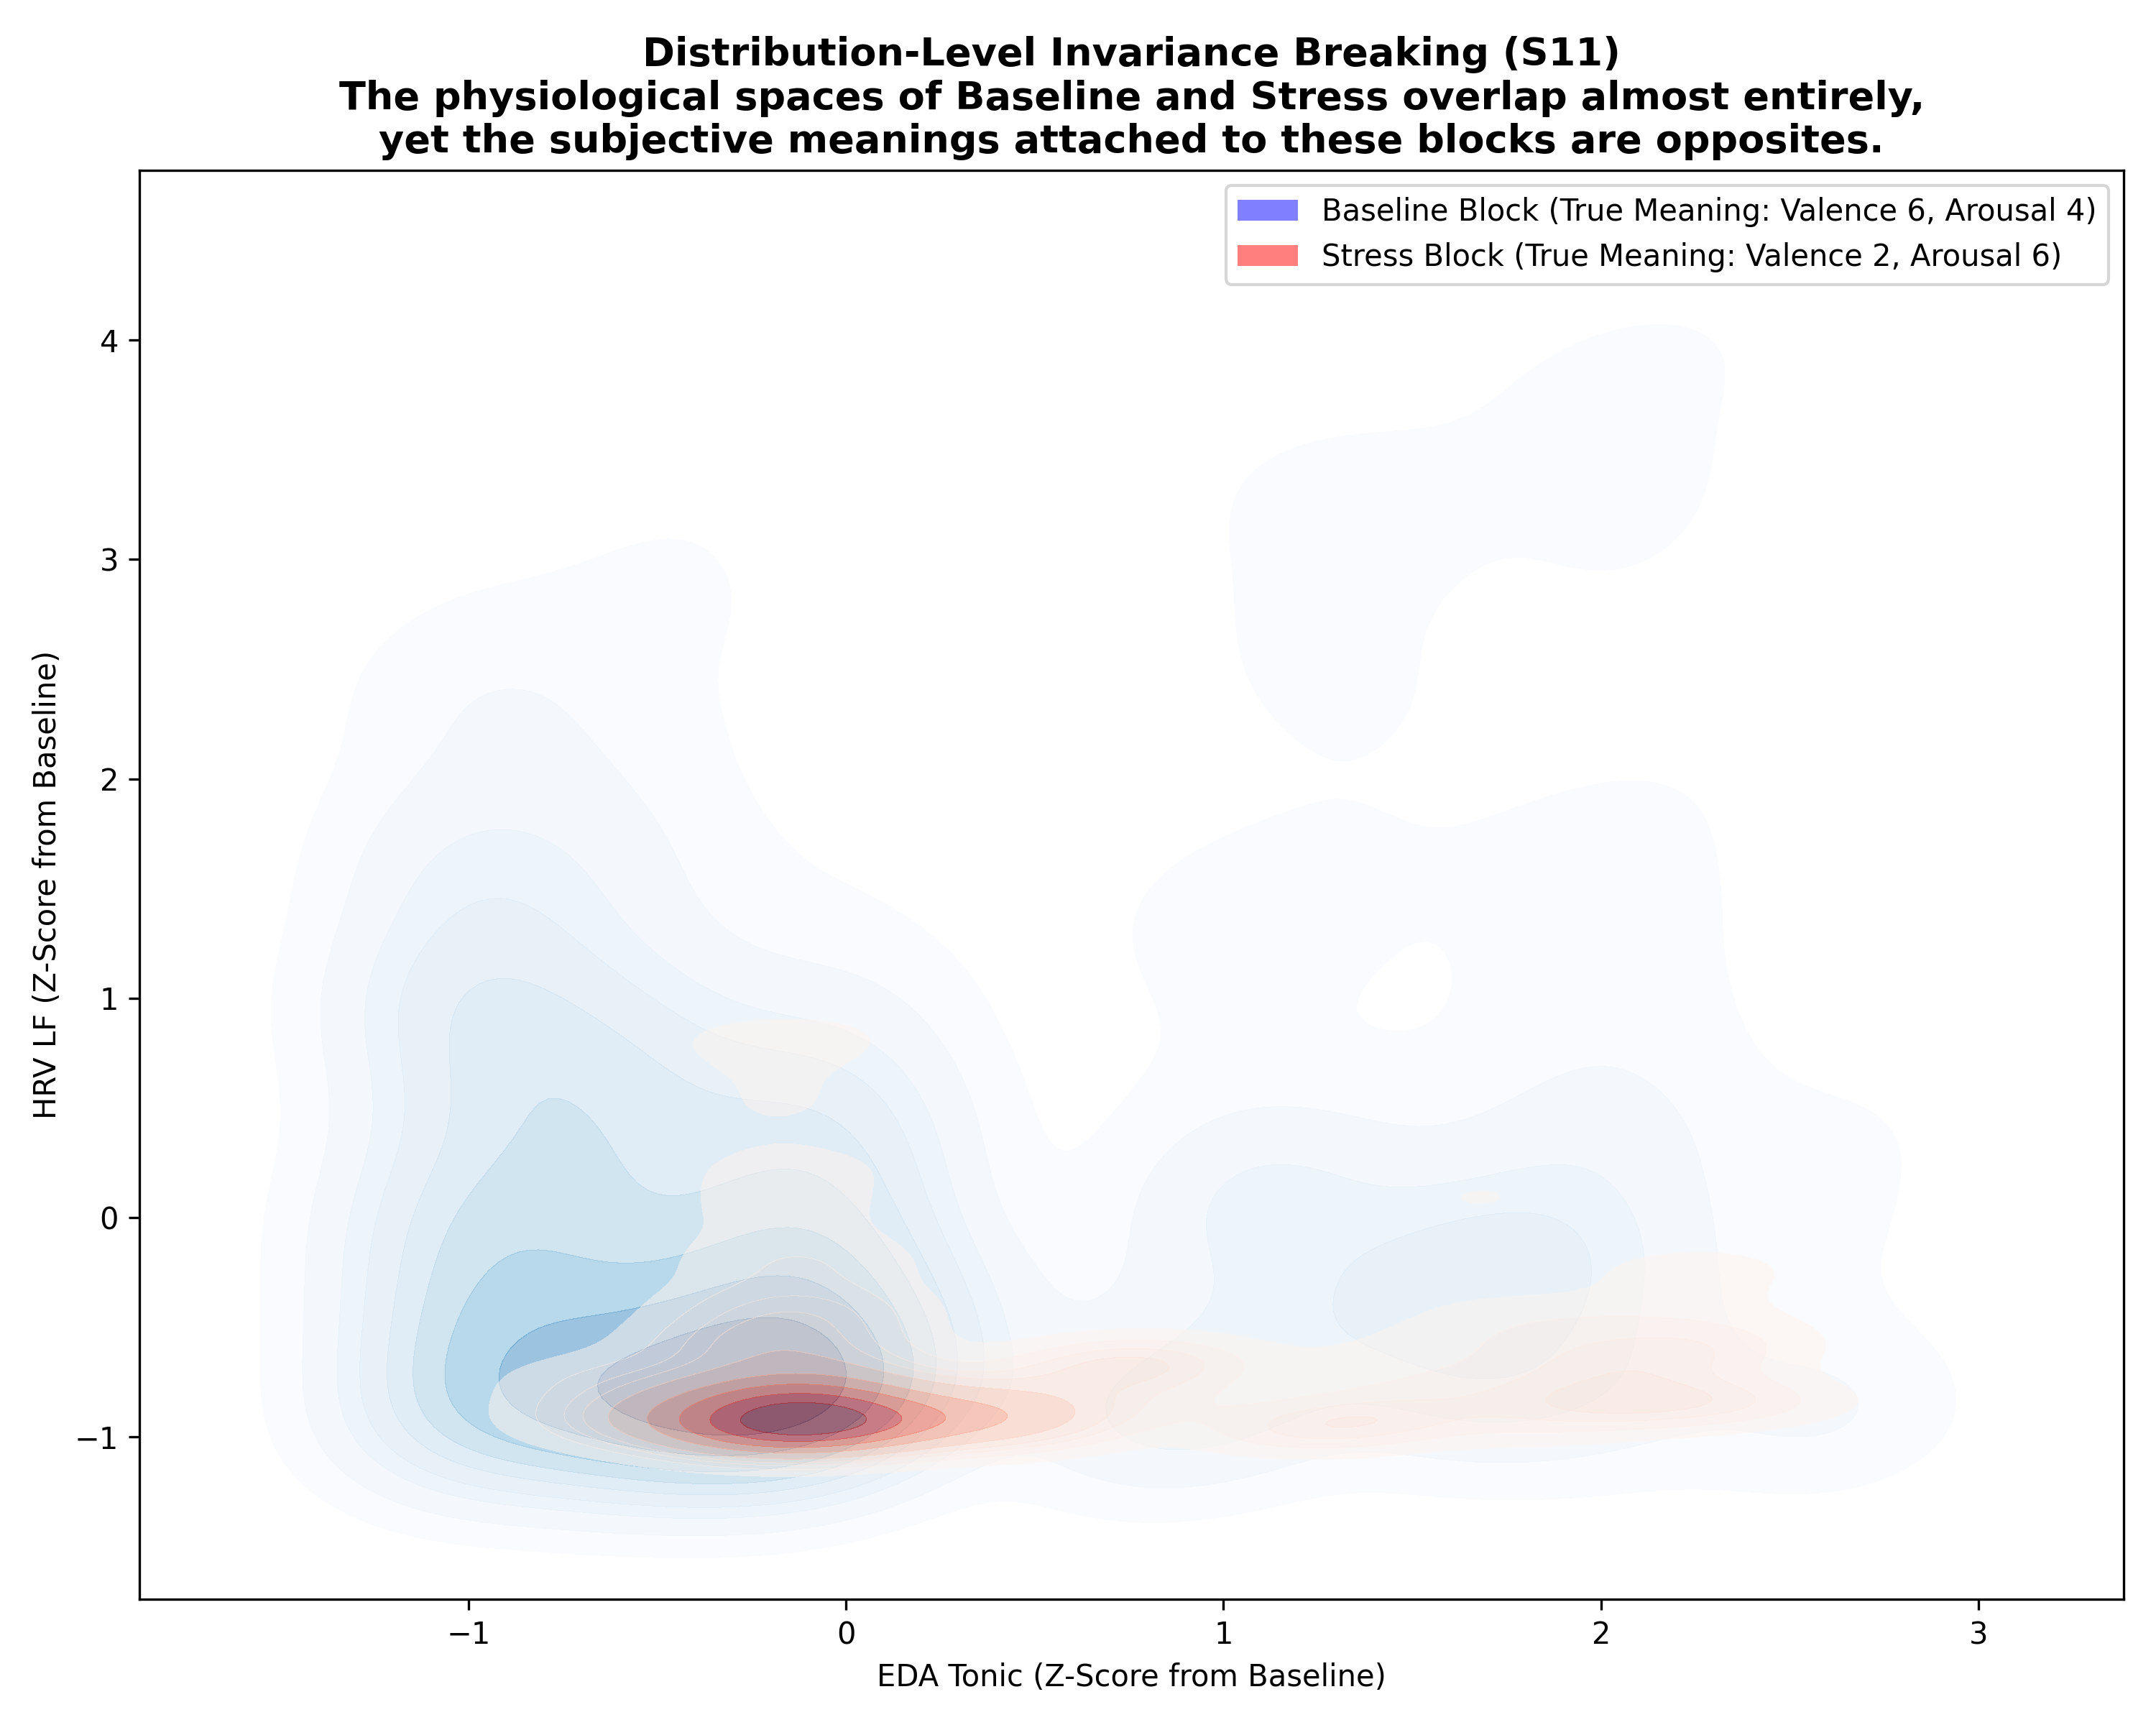
\includegraphics[width=0.45\textwidth]{distribution_overlap_S11.png}
    \caption{Distribution-Level Overlap for S11. The Baseline (blue) and Stress (red) physiological spaces overlay nearly completely, yet their respective subjective SAM scores demonstrate profound divergence (Valence 6 vs. 2).}
    \label{fig:s11}
\end{figure}

\subsection{Universality of the Invariance Breakdown}
Table \ref{tab:overlap} reports the comprehensive $\Omega$ values for all 15 subjects alongside their reported Stress task SAM Valence. 

\begin{table}[h]
\caption{Distribution Overlap ($\Omega$) and Subjective Valence during Stress Task across all WESAD Subjects.}
\label{tab:overlap}
\centering
\begin{tabular}{ccc}
\toprule
Subject ID & Overlap $\Omega$ (\%) & Stress SAM Valence (1-9) \\
\midrule
\textbf{S2} & \textbf{98.68\%} & 3 (Negative) \\
\textbf{S17} & \textbf{93.63\%} & 3 (Negative) \\
\textbf{S11} & \textbf{92.64\%} & 2 (Negative) \\
\textbf{S3} & \textbf{87.91\%} & 2 (Negative) \\
S14 & 15.76\% & 3 \\
S8 & 4.82\% & 2 \\
S7 & 3.74\% & 2 \\
S13 & 1.79\% & 2 \\
\bottomrule
\end{tabular}
\vfill
*(Subjects S4, S5, S6, S9, S10, S15, S16 exhibited $0\%$ exact overlap at the ultra-strict $1.0\sigma$ limit in 4D space, indicating strong physiological separation).*
\end{table}

The analysis reveals extreme individual differences in autonomic manifestation. In roughly 27\% of participants (S2, S17, S11, and S3), over 87\% of their active Stress-task physiology was biologically indistinguishable from their Baseline-task dimensions. Figure \ref{fig:top4} visualizes this spatial convergence.

\begin{figure}[h]
    \centering
    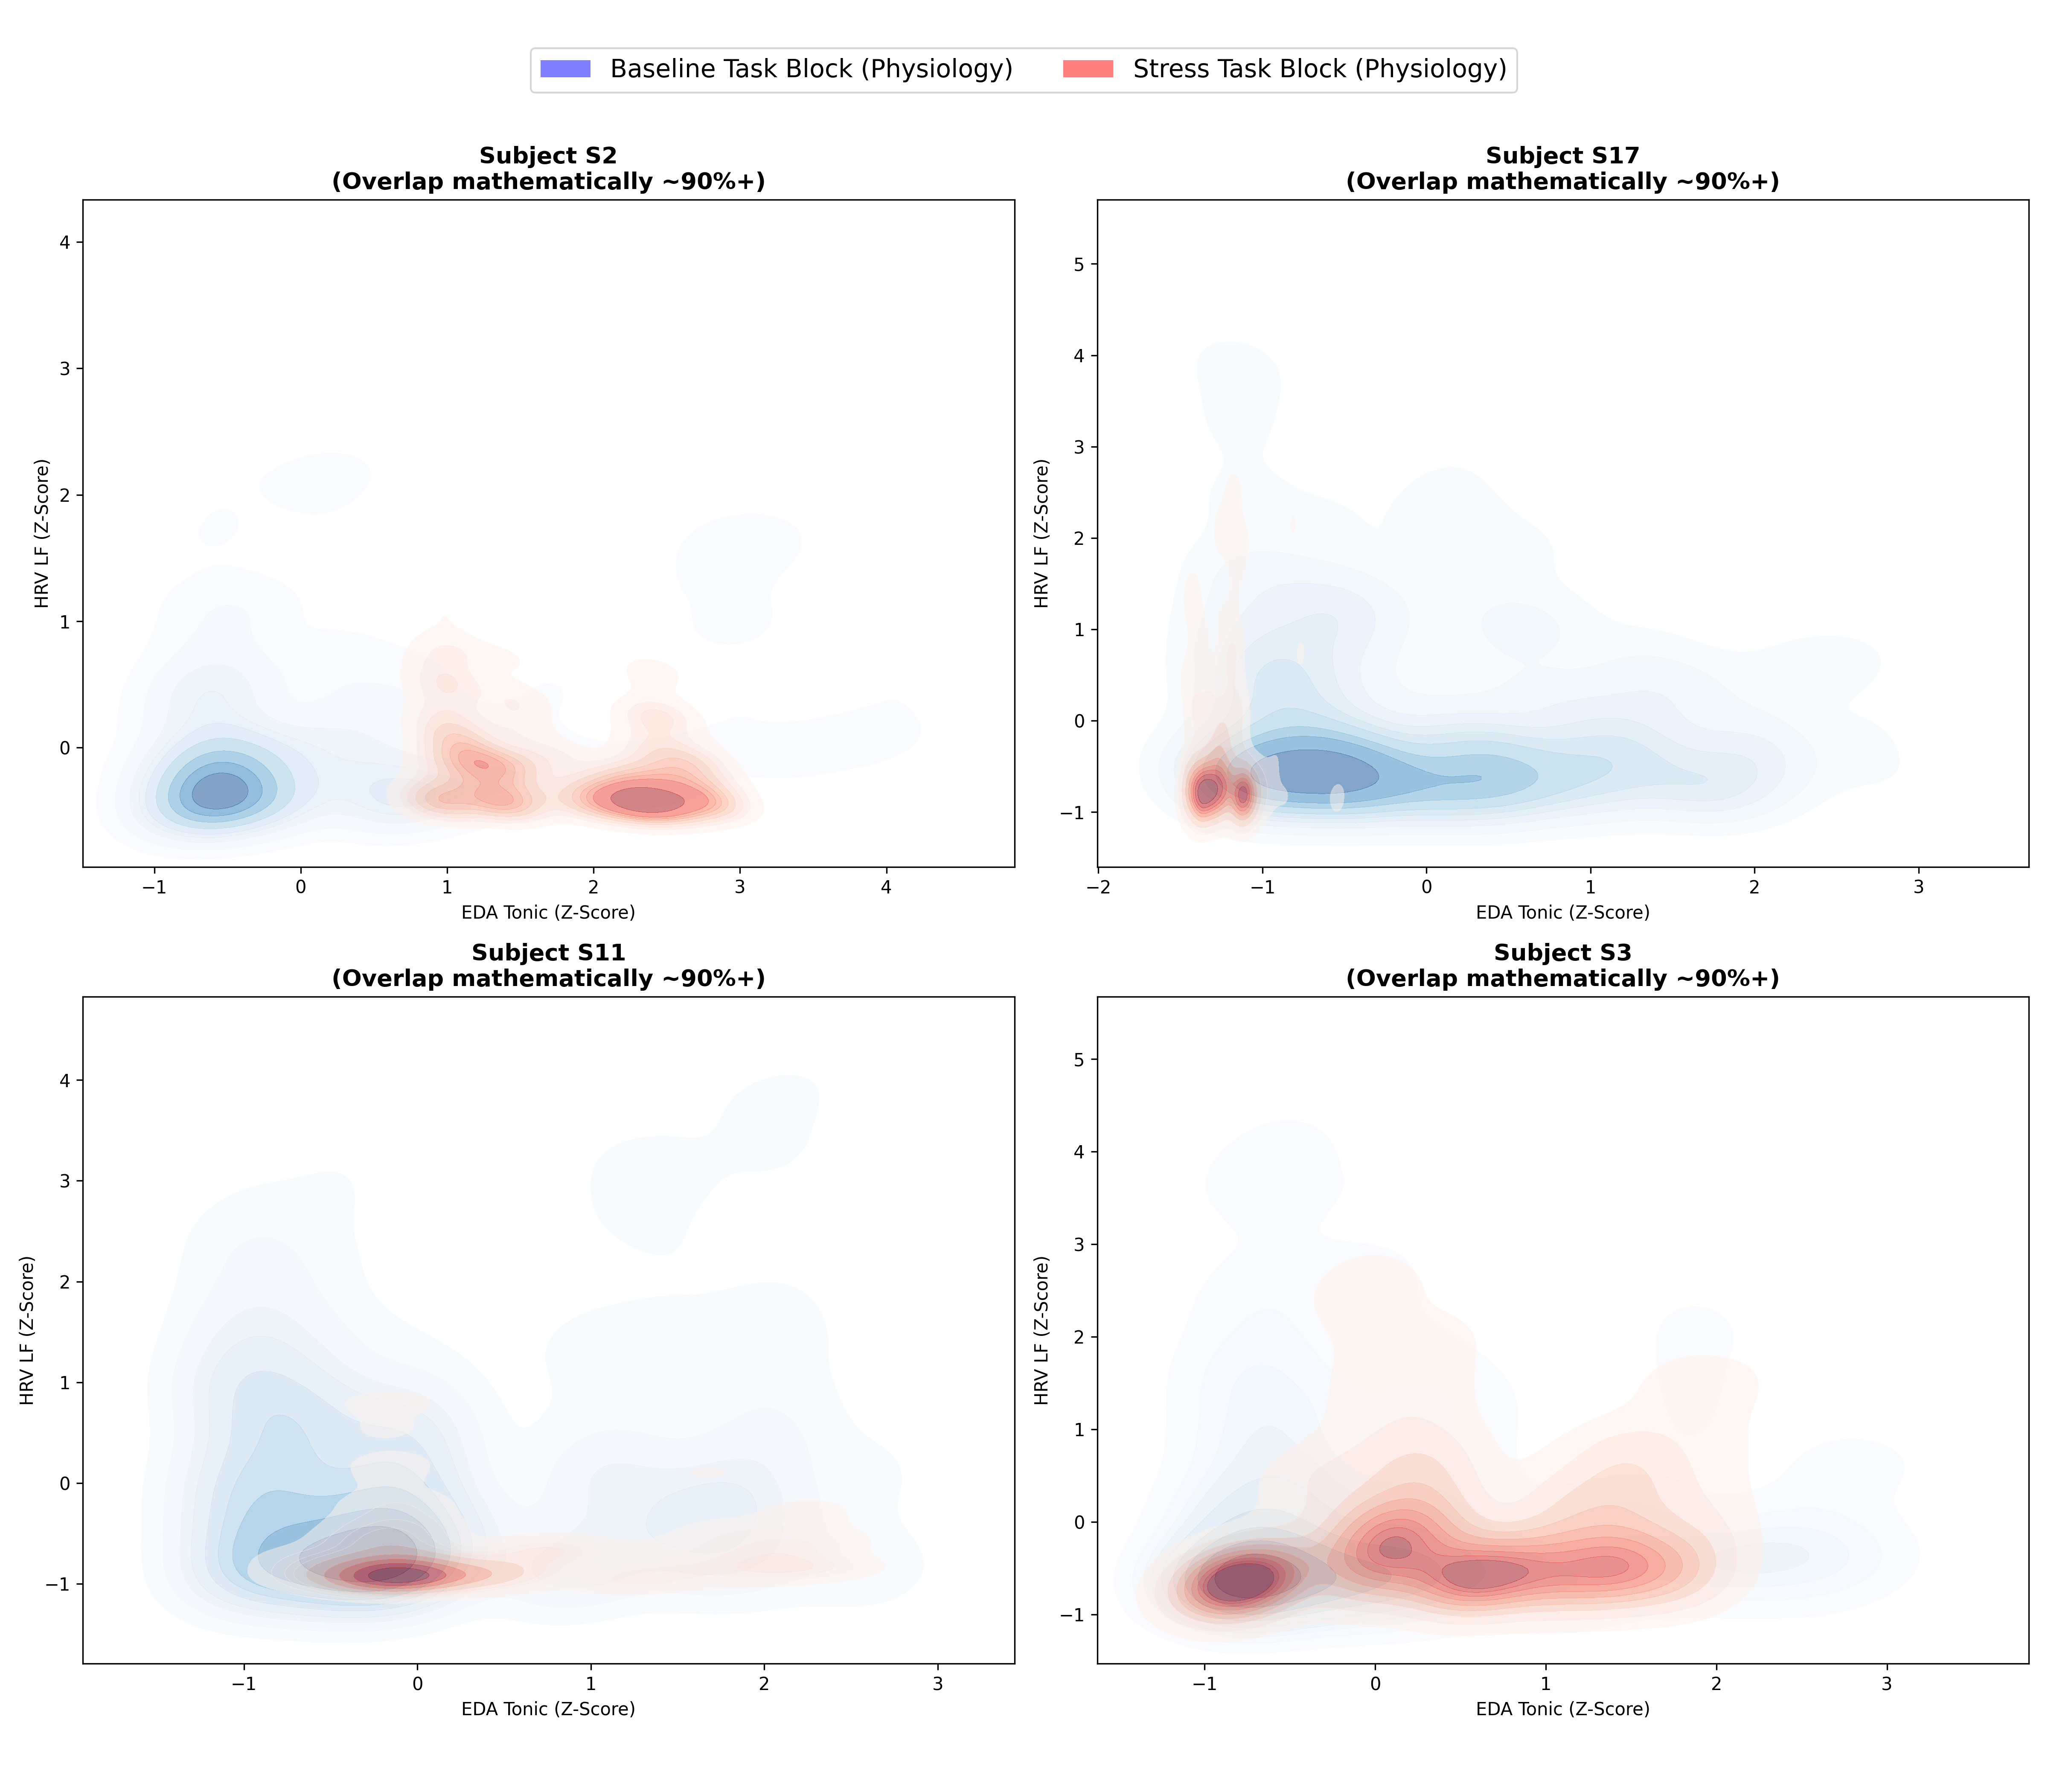
\includegraphics[width=0.48\textwidth]{top4_invariance_breaking.png}
    \caption{2D KDE physiological overlay for the top 4 overlapping subjects. Biological responses fail to separate contextual conditions.}
    \label{fig:top4}
\end{figure}

Classical supervised learning models trained to deterministically forecast subjective emotion from autonomic sensor data will inherently fail for this significant subset of the population, as the physiological prerequisite for classification is completely absent.

\section{Discussion and Conclusion}
The results empirically illuminate a severe boundary condition for contemporary ubiquitous sensing. By abolishing flawed point-level label interpolation, we computed native distribution overlaps demonstrating that physiological parameters frequently congregate in dense ``ambiguity zones'' spanning disparate contextual tasks. Because the ultimate subjective emotion separates profoundly across these physically identical states, attempting to deterministically bridge sensors directly to human feelings lacks fundamental ecological validity. 

This breakdown of physiological invariance demands a paradigm shift in human-computer interaction (HCI). Future affective systems must deprecate absolute ``state determination.'' Instead, frameworks should harness localized models, such as dynamic Gaussian Mixture Models (GMM), to identify when a user crosses into these physiological ambiguity zones. Sensing algorithms should actuate low-cognitive-load external interfaces to simply reflect autonomic shifts, dynamically delegating the final semantic interpretation (the meaning) back to the context-aware human user.

\bibliographystyle{IEEEtran}
\begin{thebibliography}{9}

\bibitem{picard1997}
R. W. Picard, \textit{Affective Computing}. MIT Press, 1997.

\bibitem{schmidt2018wesad}
P. Schmidt, A. Reiss, R. Duerichen, C. Marberger, and K. Van Laerhoven, ``Introducing WESAD, a multimodal dataset for wearable stress and affect detection,'' in \textit{Proceedings of the 20th ACM International Conference on Multimodal Interaction}, 2018, pp. 400--408.

\bibitem{bradley1994}
M. M. Bradley and P. J. Lang, ``Measuring emotion: the self-assessment manikin and the semantic differential,'' \textit{Journal of behavior therapy and experimental psychiatry}, vol. 25, no. 1, pp. 49--59, 1994.

\bibitem{wilhelm2006}
P. Wilhelm and M. Schoebi, ``Assessing mood in daily life,'' \textit{European Journal of Psychological Assessment}, vol. 23, no. 4, pp. 258--267, 2007.

\bibitem{barrett2017}
L. F. Barrett, \textit{How emotions are made: The secret life of the brain}. Houghton Mifflin Harcourt, 2017.

\bibitem{cvxeda2015}
A. Greco, G. Valenza, A. Lanata, E. P. Scilingo, and L. Citi, ``cvxEDA: A Convex Optimization Approach to Electrodermal Activity Processing,'' \textit{IEEE Transactions on Biomedical Engineering}, vol. 63, no. 4, pp. 797--804, 2016.

\end{thebibliography}

\end{document}
